\documentclass {article}
\usepackage[margin=0.5in,paperwidth=6in,paperheight=5in]{geometry}
\usepackage{ProofPower,graphicx,listings,animate}
\begin{document}

\section*{Specification:}
This is our final group project designed to demonstrate the various techniques we have learned in this course. We are specified to use a certain number of functions, as well as a minimum number of windows, various arrays, loops and images. The main requirement of the project was to collaborate as a team to test what it would be like to write a program in a professional environment. We will be using FLTK and Fluid for the graphical user interface, C++ for the body of the code, and LaTeX to document our project. Our team has decided to design and implement a "dancing" game.


Due to the time constraints of this assignment, our program, although functional, is not to the point which we would like it to be. If there were more time to add features, our team would like to have been able to include a score saving feature, as well as additional images in the start screen, help and Game Over windows. We also had intended on including extra levels with different backgrounds, a "Lives" feature, and an increasing difficulty as time in the game progressed.
\clearpage

\section*{Analysis:}

\begin{itemize}
\item Inputs: 
The inputs for this project are user triggered through button presses on the keyboard. Arrow keys, as well as mouse clicks and the space bar are all required user inputs.
\item Process: 
\begin{itemize} 
\item Decide on the over all look and layout of the final design.
\item Use the internet to find various gif, jpeg and png images to imbed in the program.
\item Write psuedo code to determine the necessary functions, loops, et cetera.
\item Collaborate as a team to code the images and various inputs in to the final program.
\end{itemize} 
\item Outputs:
The outputs for our program are the gif images which cycle regularly, as well as the pop up windows which provide the user with game play information.
\end{itemize}

\clearpage

\section*{Design}

\begin{enumerate}
\item We began by brainstorming ideas for our final design. The concept changed forms a number of times, and we eventually settled on a "Dance Dance Revolution" style matching game.
\item Next we began to write a mock up of our program using psuedo code to determine what inputs were necessary and which loops, functions, et cetera, would need to be implemented.
\item We then took to the internet to find the various gif, jpeg and png images to imbed in to the program.
\item Next we initiated the implementation of our program using FLTK to design the layout of the final design.
\item The program is designed to receive inputs from the user and recognize when the inputs match what has been displayed.
\item The program utilizes a random image generator to cycle through images of a keyboard's arrow keys.
\item When a correct (matching) key is pressed within a specified time limit, the gif image on screen cycles and a new randomly generated arrow key appears on screen.
\item If the user presses the wrong key, or allows the timer to run out on the currently displayed key, the game ends and the player has lost.
\item When the player has been eliminated, a "Game Over" prompt appears on screen and the program restarts.
\end{enumerate}

\section*{Implementation:}
Here is the code for our game. We begin by include all of the necessary header files and intiating our variables.

\begin{GFT}{C++ source code written to file dance.cpp}
\+\#include <iostream>\\
\+\#include <sstream>\\
\+\#include <stdlib.h>\\
\+\#include <time.h>\\
\+\#include "dance.h"\\
\+\\
\+Game\_Window* game\_win;\\
\+Fl\_Double\_Window* menu\_win;\\
\+Fl\_Double\_Window* help\_win;\\
\+Fl\_Double\_Window* gameover\_win;\\
\end{GFT}
\clearpage
This section of code creates an array of images we will use for our backgrounds.

\begin{GFT}{C++ source code appended to file dance.cpp}
\+Fl\_JPEG\_Image* i\_background [2];\\
\+Fl\_PNG\_Image* i\_presstostart;\\
\+Fl\_PNG\_Image* i\_key\_bg;\\
\+\\
\end{GFT}
Here is where we create our images for the arrow keys.
\begin{GFT}{C++ source code appended to file dance.cpp}
\+\\
\+Fl\_PNG\_Image* i\_key\_up;\\
\+Fl\_PNG\_Image* i\_key\_down;\\
\+Fl\_PNG\_Image* i\_key\_left;\\
\+Fl\_PNG\_Image* i\_key\_right;\\
\+\\
\end{GFT}
\clearpage
This section of code is where we do the calculation to decide wether the correct key has been pressed.
\begin{GFT}{C++ source code appended to file dance.cpp}
\+\\
\+bool correctKeyPressed = false;\\
\+bool incorrectKeyPressed = false;\\
\+int expectedKey = 0;\\
\+\\
\end{GFT}
When any event happens, this is called. "e" is the code for the type of event.
\begin{GFT}{C++ source code appended to file dance.cpp}
\+\\
\+int Game\_Window::handle(int e)\\
\+\{\\
\+	if(e == 12)\\
\+	\{\\
\+		if(Fl::event\_key() == expectedKey)\\
\+			correctKeyPressed = true;\\
\+\\
\+		else if(Fl::event\_key() == 32) // Key for spacebar\\
\end{GFT}
\clearpage
\begin{GFT}{C++ source code appended to file dance.cpp}
\+			startPlaying();\\
\+		else\\
\+		\{\\
\+			incorrectKeyPressed = true;\\
\+			correctKeyPressed = false;\\
\+		\}\\
\+		std::cout << Fl::event\_key() << std::endl;\\
\+	\}\\
\+      return 0;\\
\+\}\\
\+\\
\end{GFT}
\clearpage
Here is the function to load the background images.
\begin{GFT}{C++ source code appended to file dance.cpp}
\+\\
\+void loadBackgrounds()\\
\+\{\\
\+	i\_background[0] = new Fl\_JPEG\_Image("res/bg/bg\_1.jpg");\\
\+	i\_background[1] = new Fl\_JPEG\_Image("res/bg/bg\_2.jpg");\\
\+	\\
\+	i\_presstostart = new Fl\_PNG\_Image("res/bg/spacebar.png");\\
\+	i\_key\_bg = new Fl\_PNG\_Image("res/bg/bg\_key.png");\\
\+\}\\
\+\\
\end{GFT}
\clearpage
And the function to load the arrow keys.
\begin{GFT}{C++ source code appended to file dance.cpp}
\+\\
\+void loadArrowKeys()\\
\+\{\\
\+	i\_key\_up = new Fl\_PNG\_Image("res/keys/up\_key.png");\\
\+	i\_key\_down = new Fl\_PNG\_Image("res/keys/down\_key.png");\\
\+	i\_key\_left = new Fl\_PNG\_Image("res/keys/left\_key.png");\\
\+	i\_key\_right = new Fl\_PNG\_Image("res/keys/right\_key.png");\\
\+\}\\
\+\\
\end{GFT}
\clearpage
Here, we initiate the arrays for oading the various frames of the GIF images.

\begin{GFT}{C++ source code appended to file dance.cpp}
\+\\
\+const int carlton\_N = 24;\\
\+const int justin\_N = 25;\\
\+const int mj\_N = 9;\\
\+const int snoop\_N = 19;\\
\+Fl\_GIF\_Image* carlton\_images[carlton\_N]; // frames are 0-23\\
\+Fl\_GIF\_Image* justin\_images[justin\_N]; // frames are 0-24\\
\+Fl\_GIF\_Image* mj\_images[mj\_N]; // frames are 0-8\\
\+Fl\_GIF\_Image* snoop\_images[snoop\_N]; // frames are 0-18\\
\+\\
\end{GFT}
\clearpage
These functions are responsible for the actual loading and cycling of the GIF images. 

\begin{GFT}{C++ source code appended to file dance.cpp}
\+\\
\+void loadGifs()\\
\+\{\\
\+     for(int i = 0; i < carlton\_N; i++)\\
\+     \{\\
\+       std::ostringstream oss;\\
\+       oss << "res/dancers/carlton/carlton" << i << ".gif";\\
\+       carlton\_images[i] = new Fl\_GIF\_Image(oss.str().c\_str());\\
\+     \}\\
\+\\
\+     for(int i = 0; i < justin\_N; i++)\\
\+     \{\\
\+       std::ostringstream oss;\\
\+       oss << "res/dancers/justin/justin" << i << ".gif";\\
\+       justin\_images[i] = new Fl\_GIF\_Image(oss.str().c\_str());\\
\+     \}\\
\end{GFT}
\clearpage
\begin{GFT}{C++ source code appended to file dance.cpp}
\+\\
\+     for(int i = 0; i < mj\_N; i++)\\
\+     \{\\
\+       std::ostringstream oss;\\
\+       oss << "res/dancers/michael/mj" << i << ".gif";\\
\+       mj\_images[i] = new Fl\_GIF\_Image(oss.str().c\_str());\\
\+     \}\\
\+\\
\+     for(int i = 0; i < snoop\_N; i++)\\
\+     \{\\
\+       std::ostringstream oss;\\
\+       oss << "res/dancers/snoop/snoop" << i << ".gif";\\
\+       snoop\_images[i] = new Fl\_GIF\_Image(oss.str().c\_str());\\
\+     \}\\
\+ \\
\+\}\\
\end{GFT}
\clearpage
\begin{GFT}{C++ source code appended to file dance.cpp}
\+void animate\_carlton(void*)\\
\+\{\\
\+     static int i = 0;\\
\+     game\_win->carlton->image(carlton\_images[i]);\\
\+     game\_win->carlton->parent()->redraw();\\
\+     i = (i + 1) \% carlton\_N;\\
\+     Fl::repeat\_timeout(.075,animate\_carlton);\\
\+\}\\
\+void animate\_justin(void*)\\
\+\{\\
\+     static int i = 0;\\
\+     game\_win->carlton->hide();\\
\+     game\_win->justin->image(justin\_images[i]);\\
\+     game\_win->justin->parent()->redraw();\\
\+     i = (i + 1) \% justin\_N;\\
\+     Fl::repeat\_timeout(.075,animate\_justin);\\
\+\}\\
\end{GFT}
\clearpage
\begin{GFT}{C++ source code appended to file dance.cpp}
\+void animate\_mj(void*)\\
\+\{\\
\+     static int i = 0;\\
\+     game\_win->justin->hide();\\
\+     game\_win->mj->image(mj\_images[i]);\\
\+     game\_win->mj->parent()->redraw();\\
\+     i = (i + 1) \% mj\_N;\\
\+     Fl::repeat\_timeout(.075,animate\_mj);\\
\+\}\\
\+void animate\_snoop(void*)\\
\+\{\\
\+     static int i = 0;\\
\+     game\_win->mj->hide();\\
\+     game\_win->snoop->image(snoop\_images[i]);\\
\+     game\_win->snoop->parent()->redraw();\\
\+     i = (i + 1) \% snoop\_N;\\
\+     Fl::repeat\_timeout(.075,animate\_snoop);\\
\+\}\\
\end{GFT}
\clearpage
\begin{GFT}{C++ source code appended to file dance.cpp}
\+void loadImages()\\
\+\{\\
\+	loadBackgrounds();\\
\+	loadArrowKeys();\\
\+	loadGifs();\\
\+\}\\
\+\\
\end{GFT}
This part of the code loads a new lever when the player selects the start button from the GUI.

\begin{GFT}{C++ source code appended to file dance.cpp}
\+void loadLevel(int levelNum)\\
\+\{\\
\+	game\_win->box\_background->image(i\_background[levelNum]);\\
\+	\\
\+\}\\
\+\\
\end{GFT}
\clearpage
This section is where the arrow keys are randomly generated. The code is designed in such a way that the same arrow key will never present itself more than once in a row.

\begin{GFT}{C++ source code appended to file dance.cpp}
\+\\
\+void popupRandomArrow()\\
\+\{\\
\+	static int lastNum = 0;\\
\+\\
\+	int randNum = randNum = rand() \% 4 + 1;\\
\+\\
\+	while(randNum == lastNum)\\
\+		randNum = rand() \% 4 + 1;\\
\+	lastNum = randNum;\\
\+	Fl\_PNG\_Image* newArrow;\\
\end{GFT}
\clearpage
\begin{GFT}{C++ source code appended to file dance.cpp}
\+\\
\+	if(randNum == 1)\\
\+	\{\\
\+		newArrow = i\_key\_up;\\
\+		expectedKey = 65362; \\
\+	\}\\
\+	else if(randNum == 2)\\
\+	\{\\
\+		newArrow = i\_key\_down;\\
\+		expectedKey = 65364;\\
\+	\}\\
\+	else if(randNum == 3)\\
\+	\{\\
\+		newArrow = i\_key\_left;\\
\+		expectedKey = 65361;\\
\+	\}\\
\end{GFT}
\clearpage
\begin{GFT}{C++ source code appended to file dance.cpp}
\+\\
\+	else\\
\+	\{\\
\+		newArrow = i\_key\_right;\\
\+		expectedKey = 65363;\\
\+	\}\\
\+\\
\+\\
\+	game\_win->box\_key->show();\\
\+	game\_win->box\_key->image(newArrow);\\
\+	game\_win->redraw();\\
\+\}\\
\+\\
\end{GFT}
\clearpage
The following code is what actually interacts with the game player. It contains the timer which will default to a "Game Over" screen when it has expired, as well as the functions to detect if the correct key has been pressed, if the incorrect key has been pressed, of if no keys were pressed.

\begin{GFT}{C++ source code appended to file dance.cpp}
\+\\
\+void timerExpire(void*);\\
\+\\
\+void setNewTimer()\\
\+\{\\
\+	correctKeyPressed = false;\\
\+	popupRandomArrow();\\
\+	Fl::remove\_timeout(timerExpire);\\
\+	Fl::add\_timeout(1.0, timerExpire);\\
\+\}\\
\+\\
\+void timerExpire(void*)\\
\+\{\\
\+	std::cout << "Correct Key Pressed: " << correctKeyPressed << std::endl;\\
\+		std::cout << "Incorrect Key Pressed: " << incorrectKeyPressed << std::endl;\\
\end{GFT}
\clearpage
\begin{GFT}{C++ source code appended to file dance.cpp}
\+	if(incorrectKeyPressed)\\
\+	\{\\
\+		gameOver();\\
\+	\}\\
\+\\
\+	if(correctKeyPressed)\\
\+	\{\\
\+ 		setNewTimer();\\
\+		//Fl::repeat\_timeout(1.0, timerExpire);\\
\+	\}\\
\+	else\\
\+	\{	\\
\+		gameOver();\\
\+	\}\\
\+	\\
\+\}\\
\+\\
\end{GFT}
\clearpage
Here we set up all of the functions necessary to actually play the game.

\begin{GFT}{C++ source code appended to file dance.cpp}
\+\\
\+void initRandomSeed()\\
\+\{\\
\+	srand(time(NULL));\\
\+\}\\
\+\\
\+void beginKeypressSequence(void*)\\
\+\{\\
\+	setNewTimer();\\
\+	//Fl::add\_timeout(1.0, timerExpire);\\
\+\}\\
\+\\
\+void loadGameWindow()\\
\+\{\\
\+	loadImages();\\
\+	loadLevel(0);\\
\end{GFT}
\clearpage
\begin{GFT}{C++ source code appended to file dance.cpp}
\+	game\_win->box\_presstostart->image(i\_presstostart);\\
\+\\
\+	game\_win->show();\\
\+\\
\+\}\\
\+\\
\end{GFT}
\clearpage
This is where the spacebar is set to start the game when pressed.

\begin{GFT}{C++ source code appended to file dance.cpp}
\+\\
\+void startPlaying()\\
\+\{\\
\+	Fl::add\_timeout(0.2, beginKeypressSequence);\\
\+	game\_win->box\_presstostart->image(i\_key\_bg);\\
\+\\
\+	Fl::add\_timeout(0,animate\_carlton);\\
\+	Fl::add\_timeout(10,animate\_justin);\\
\+	Fl::add\_timeout(20,animate\_mj);\\
\+	Fl::add\_timeout(30,animate\_snoop);	\\
\+\}\\
\+\\
\end{GFT}
\clearpage
This function removes everything and kills the program once the player has lost the game.

\begin{GFT}{C++ source code appended to file dance.cpp}
\+\\
\+void gameOver()\\
\+\{\\
\+	/*Fl::remove\_timeout(animate\_carlton);\\
\+	Fl::remove\_timeout(animate\_carlton);\\
\+	Fl::remove\_timeout(animate\_carlton);\\
\+	Fl::remove\_timeout(animate\_carlton);*/\\
\+\\
\+	game\_win->box\_presstostart->image(i\_presstostart);\\
\+	game\_win->box\_key->hide();\\
\+\\
\+	game\_win->hide();\\
\+	gameover\_win->show();\\
\+\}\\
\+\\
\end{GFT}
\clearpage
And finally, the main function to put it all together and make it a useable program!

\begin{GFT}{C++ source code appended to file dance.cpp}
\+\\
\+int main()\\
\+\{\\
\+	game\_win = make\_game\_window();\\
\+\\
\+	menu\_win = make\_menu\_window();\\
\+	menu\_win->show();\\
\+\\
\+	help\_win = make\_help\_window();\\
\+	gameover\_win = make\_gameover\_window();\\
\+\\
\+	initRandomSeed();\\
\+\\
\+	Fl::run();\\
\+\}\\
\+\\
\end{GFT}
\clearpage
\subsection*{GUI Code:}
\lstinputlisting{dance.cxx}

\clearpage

\subsection*{Actual Output}

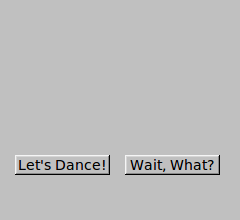
\includegraphics[scale=0.5]{dance01.png}
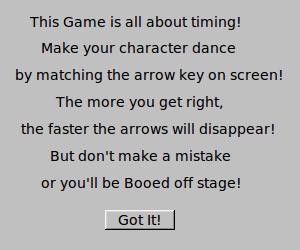
\includegraphics[scale=0.5]{dance02.png}

\clearpage

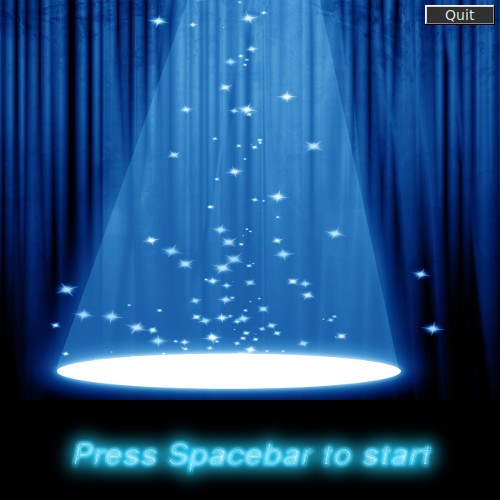
\includegraphics[scale=0.5]{dance03.png}

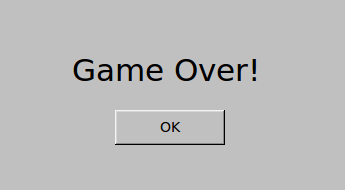
\includegraphics[scale=0.5]{dance04.png}

\clearpage
\subsection*{Proof it works}

\animategraphics[height=3in,controls]{1}{dancing}{0}{29}

\end{document}


